% !TEX program = pdflatex
% !TeX spellcheck = en_US
\documentclass[11pt,a4paper]{article}

\usepackage[utf8]{inputenc}
\usepackage[T1]{fontenc}
\usepackage{amsmath}
\usepackage{amsfonts}
\usepackage{amssymb}
\usepackage{graphicx}
\usepackage{booktabs}
\usepackage[table]{xcolor}
\usepackage[breaklinks=true,colorlinks=true,linkcolor=blue,urlcolor=blue,citecolor=blue]{hyperref}
\usepackage{caption}
\usepackage{subcaption}
\usepackage{float}
\usepackage{array}
\usepackage{enumitem}
\usepackage{microtype}
\usepackage{multirow}
\usepackage{geometry}
\geometry{a4paper, margin=2.5cm}

\title{\textbf{Audio Feature Analysis for Sound Event Detection}}
\author{Mark Sere}
\date{April 2025}

\begin{document}

\maketitle

\section{Introduction}

This report presents an analysis of audio features extracted from the MLPC2025 dataset for sound event detection.

\section{Dataset Details}

\subsection{Spectrograms and Mel Spectrograms}

\begin{figure}[H]
    \centering
    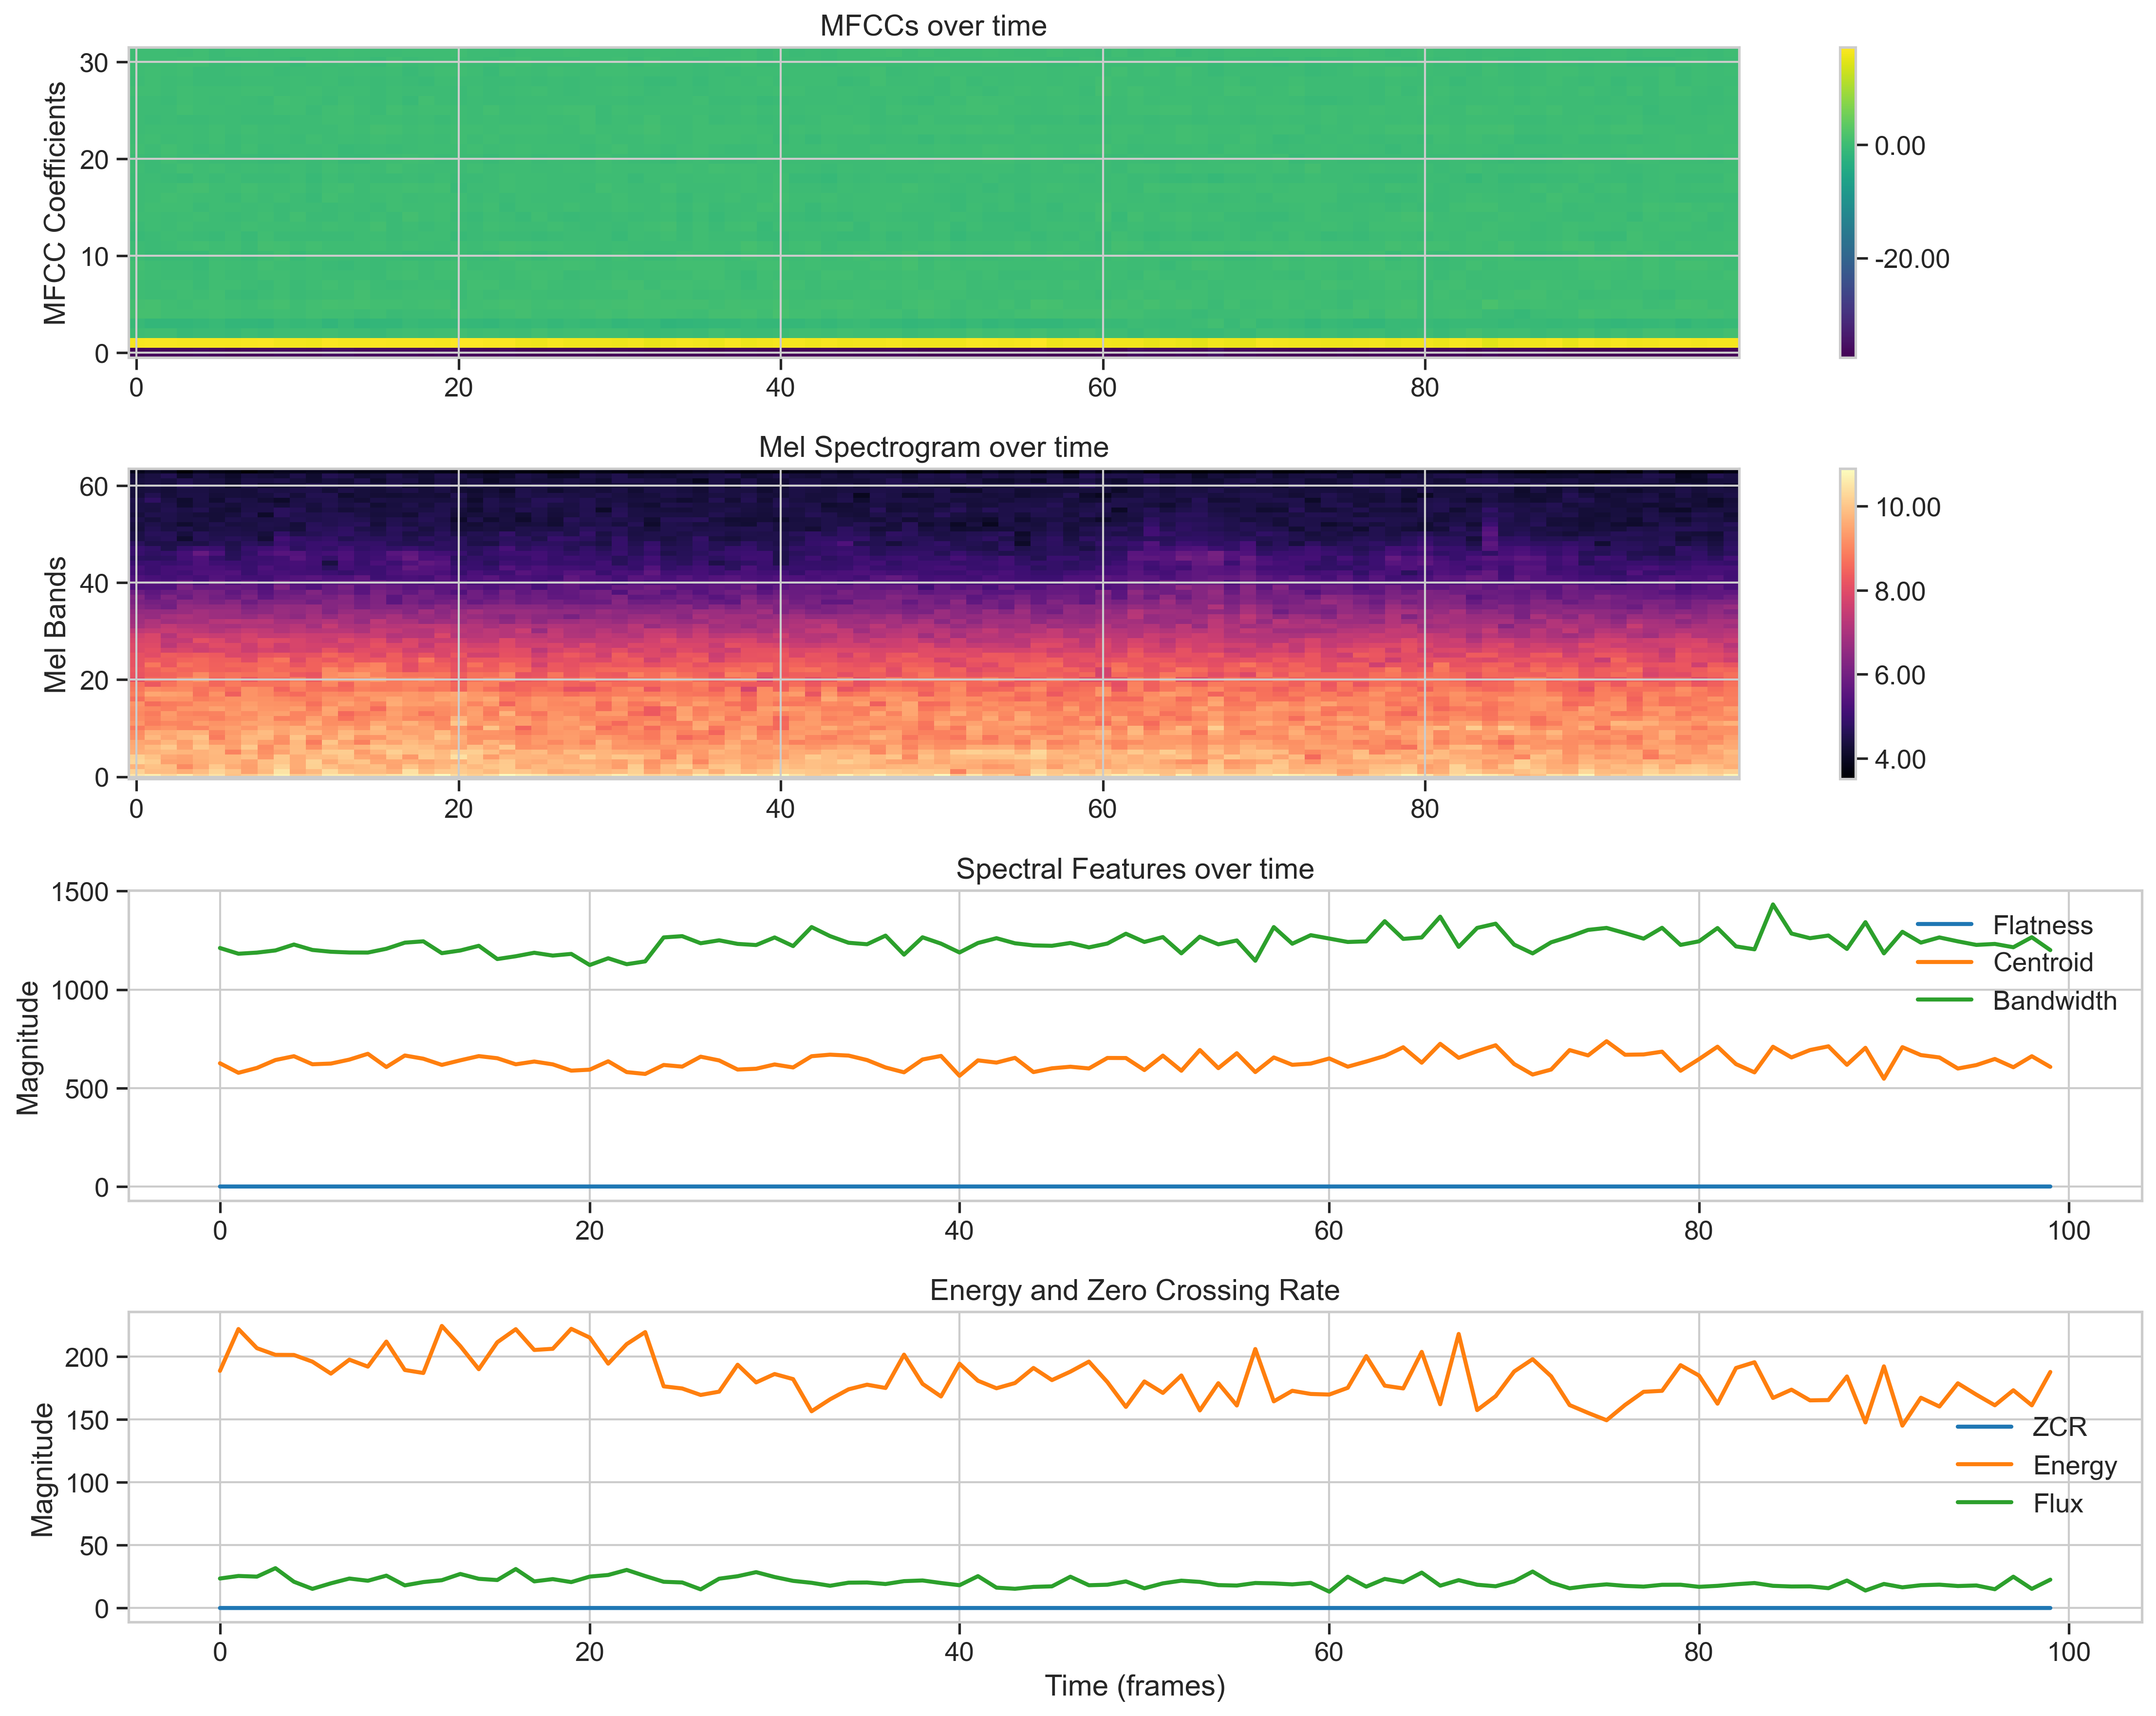
\includegraphics[width=0.8\textwidth]{audio_features_visualization.png}
    \caption{Visualization of different audio features over time for a sample file, including Mel spectrogram (second panel), which shows the distribution of energy across different frequency bands.}
    \label{fig:feature_viz}
\end{figure}

\section{Feature Analysis}

\subsection{Dimensionality Reduction}

Given the high dimensionality of the feature space (942 dimensions), Principal Component Analysis (PCA) was applied to reduce dimensionality while preserving the most important information.

\begin{figure}[H]
    \centering
    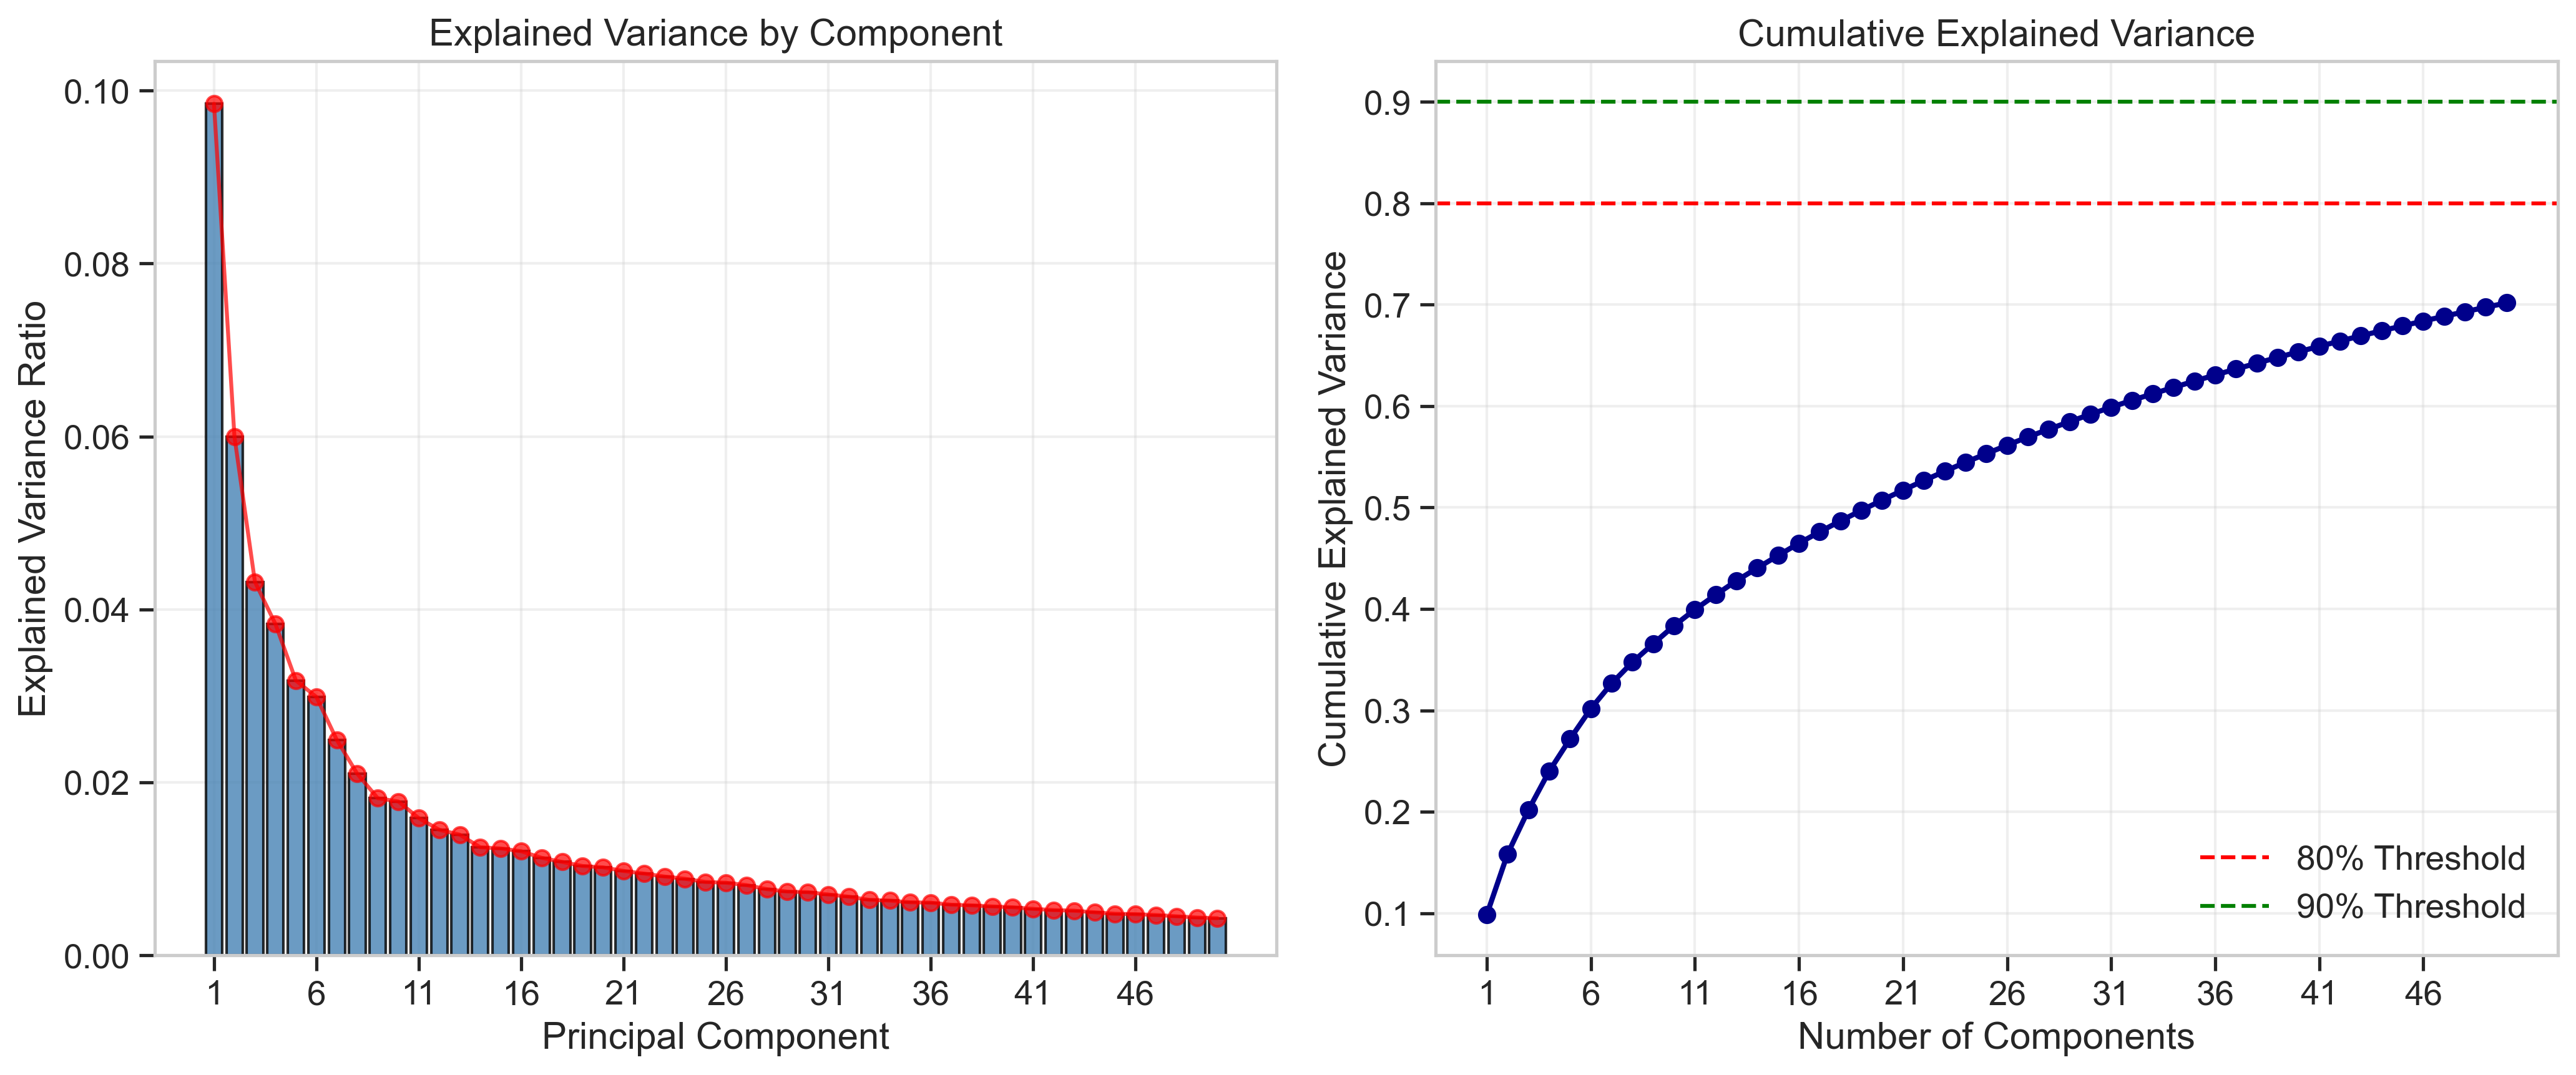
\includegraphics[width=0.95\textwidth]{pca_explained_variance.png}
    \caption{Explained variance by PCA components. Left: Individual variance contribution of each component. Right: Cumulative explained variance with 80\% and 90\% thresholds marked.}
    \label{fig:pca_variance}
\end{figure}

Analysis of the cumulative explained variance revealed that:
\begin{itemize}
    \item 82 principal components are sufficient to explain 80\% of the variance
    \item 146 components are needed to explain 90\% of the variance
\end{itemize}

This represents a significant dimensionality reduction (from 942 to 82 dimensions, or 91.3\% reduction) while maintaining most of the information content. The reduced feature set was used for subsequent clustering analysis.

\subsection{Feature Importance}

To understand which features contribute most to the principal components, the feature loadings for the top three components were analyzed.

\begin{figure}[H]
    \centering
    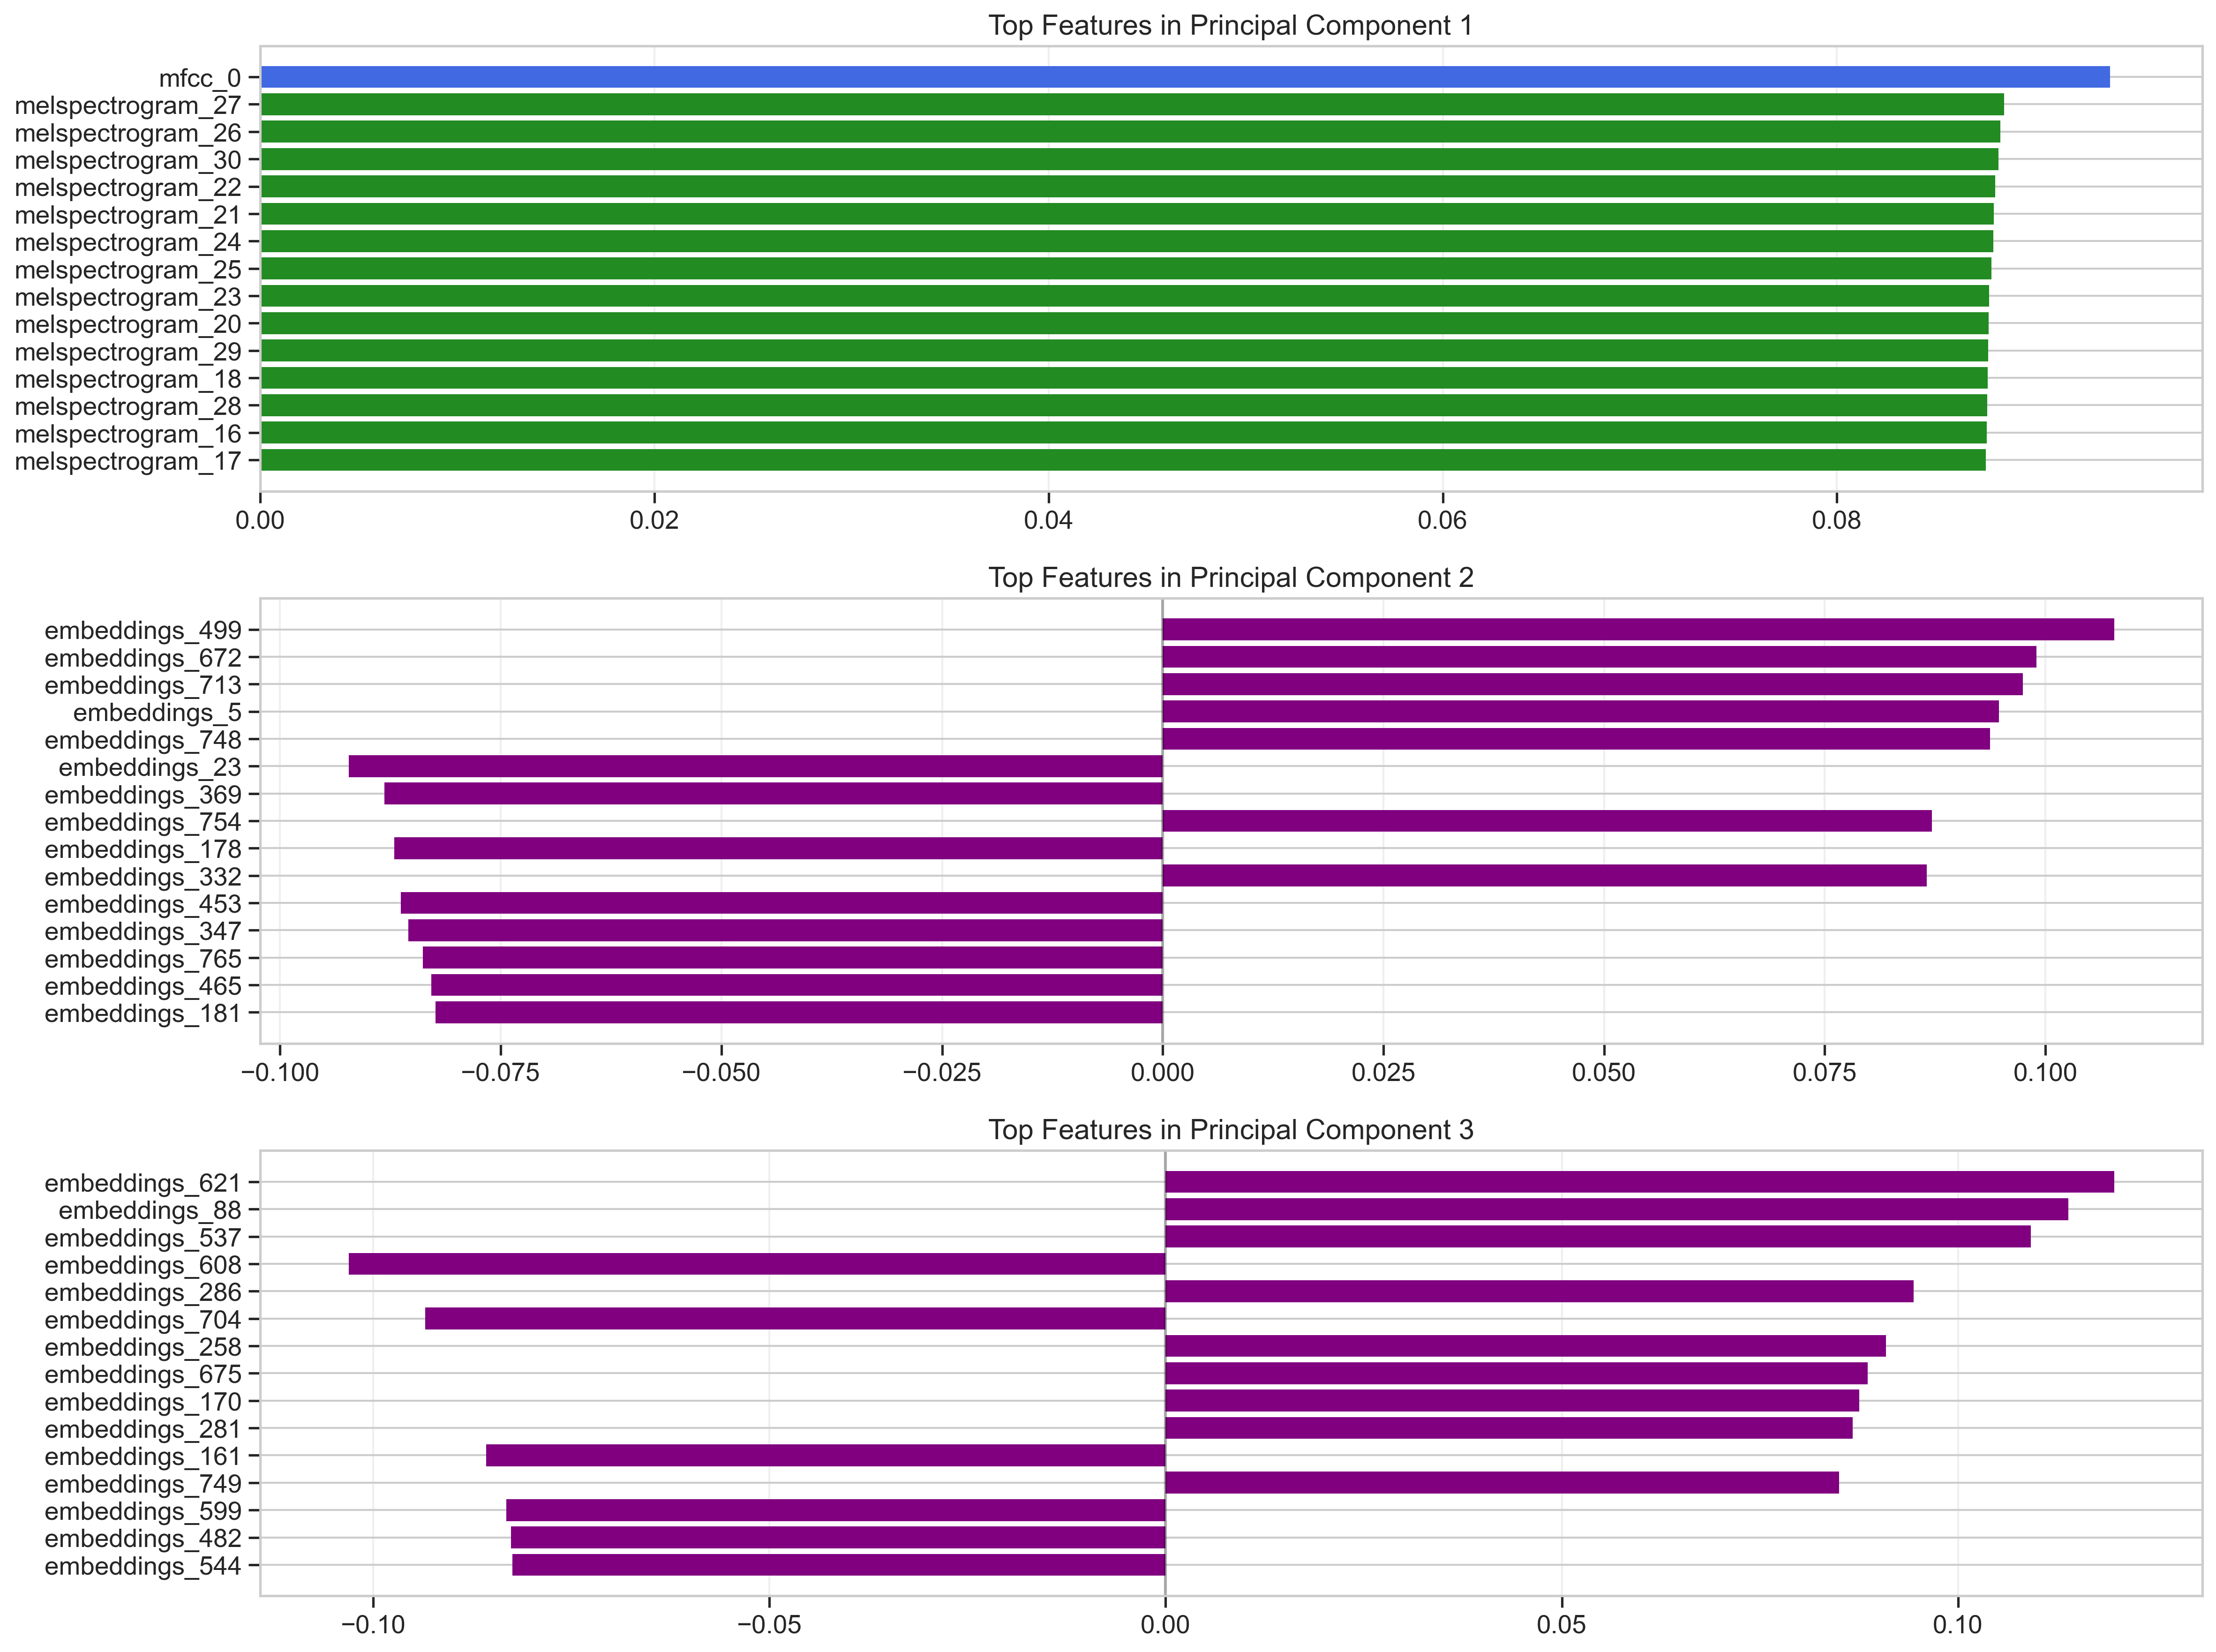
\includegraphics[width=0.95\textwidth]{feature_importance.png}
    \caption{Top 15 features contributing to the first three principal components, showing the relative importance of different feature types.}
    \label{fig:feature_importance}
\end{figure}

The analysis revealed:
\begin{itemize}
    \item \textbf{First principal component}: Dominated by Mel spectrogram features with MFCC\_0 (the DC component) having the highest loading. This suggests that energy distribution across frequency bands is the most significant factor for distinguishing audio signals.
    
    \item \textbf{Second and third principal components}: Heavily influenced by embedding features from the pre-trained neural network. These components likely capture higher-level semantic information about the audio content.
\end{itemize}

Across the top three components, the most important feature types were:
\begin{itemize}
    \item Embeddings: 30 occurrences
    \item Mel spectrogram features: 14 occurrences
    \item MFCCs: 1 occurrence
\end{itemize}

This suggests that while traditional spectral features like MFCCs are valuable, the learned embeddings capture additional information that contributes significantly to the variance in the data.

\subsection{Clustering Analysis}

K-means clustering was applied to the dimensionally-reduced feature vectors to identify natural groupings in the audio data. To determine the optimal number of clusters, silhouette scores were calculated for different values of k.

\begin{figure}[H]
    \centering
    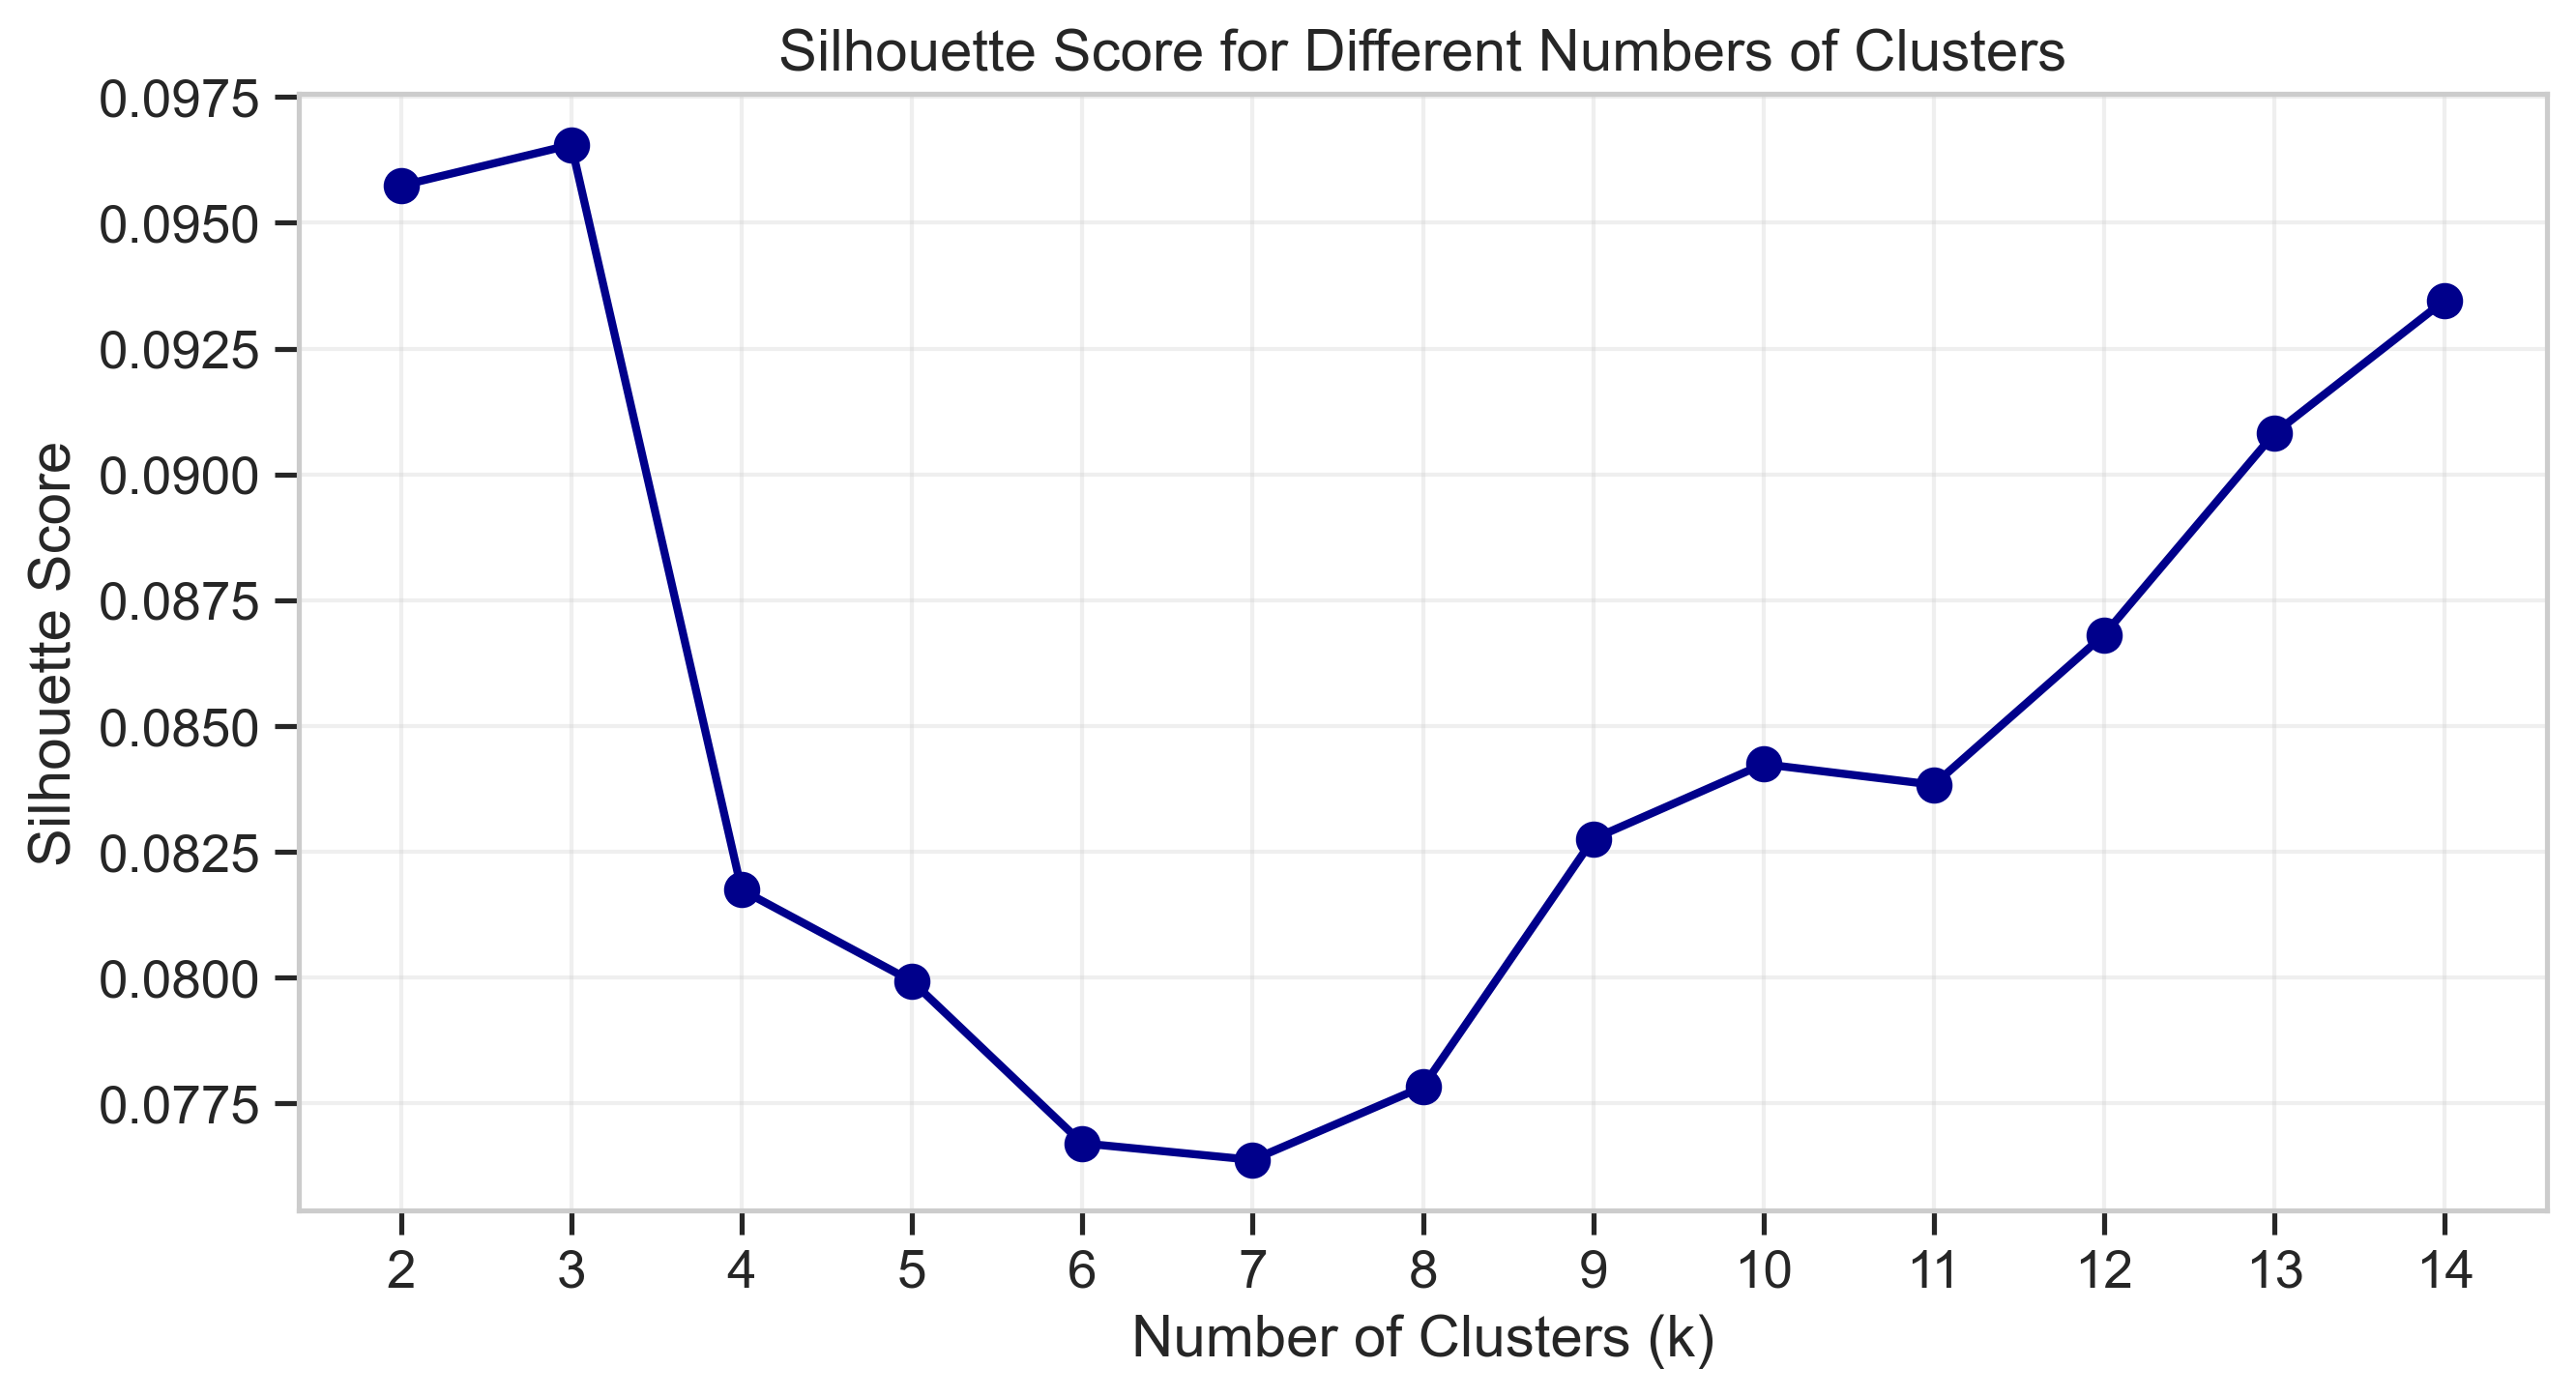
\includegraphics[width=0.7\textwidth]{silhouette_scores.png}
    \caption{Silhouette scores for different numbers of clusters (k), showing that k=3 provides the best cluster separation.}
    \label{fig:silhouette}
\end{figure}

The silhouette analysis indicated that 3 clusters provided the optimal balance between cluster separation and cohesion. The dataset was subsequently partitioned into these three clusters.

\begin{figure}[H]
    \centering
    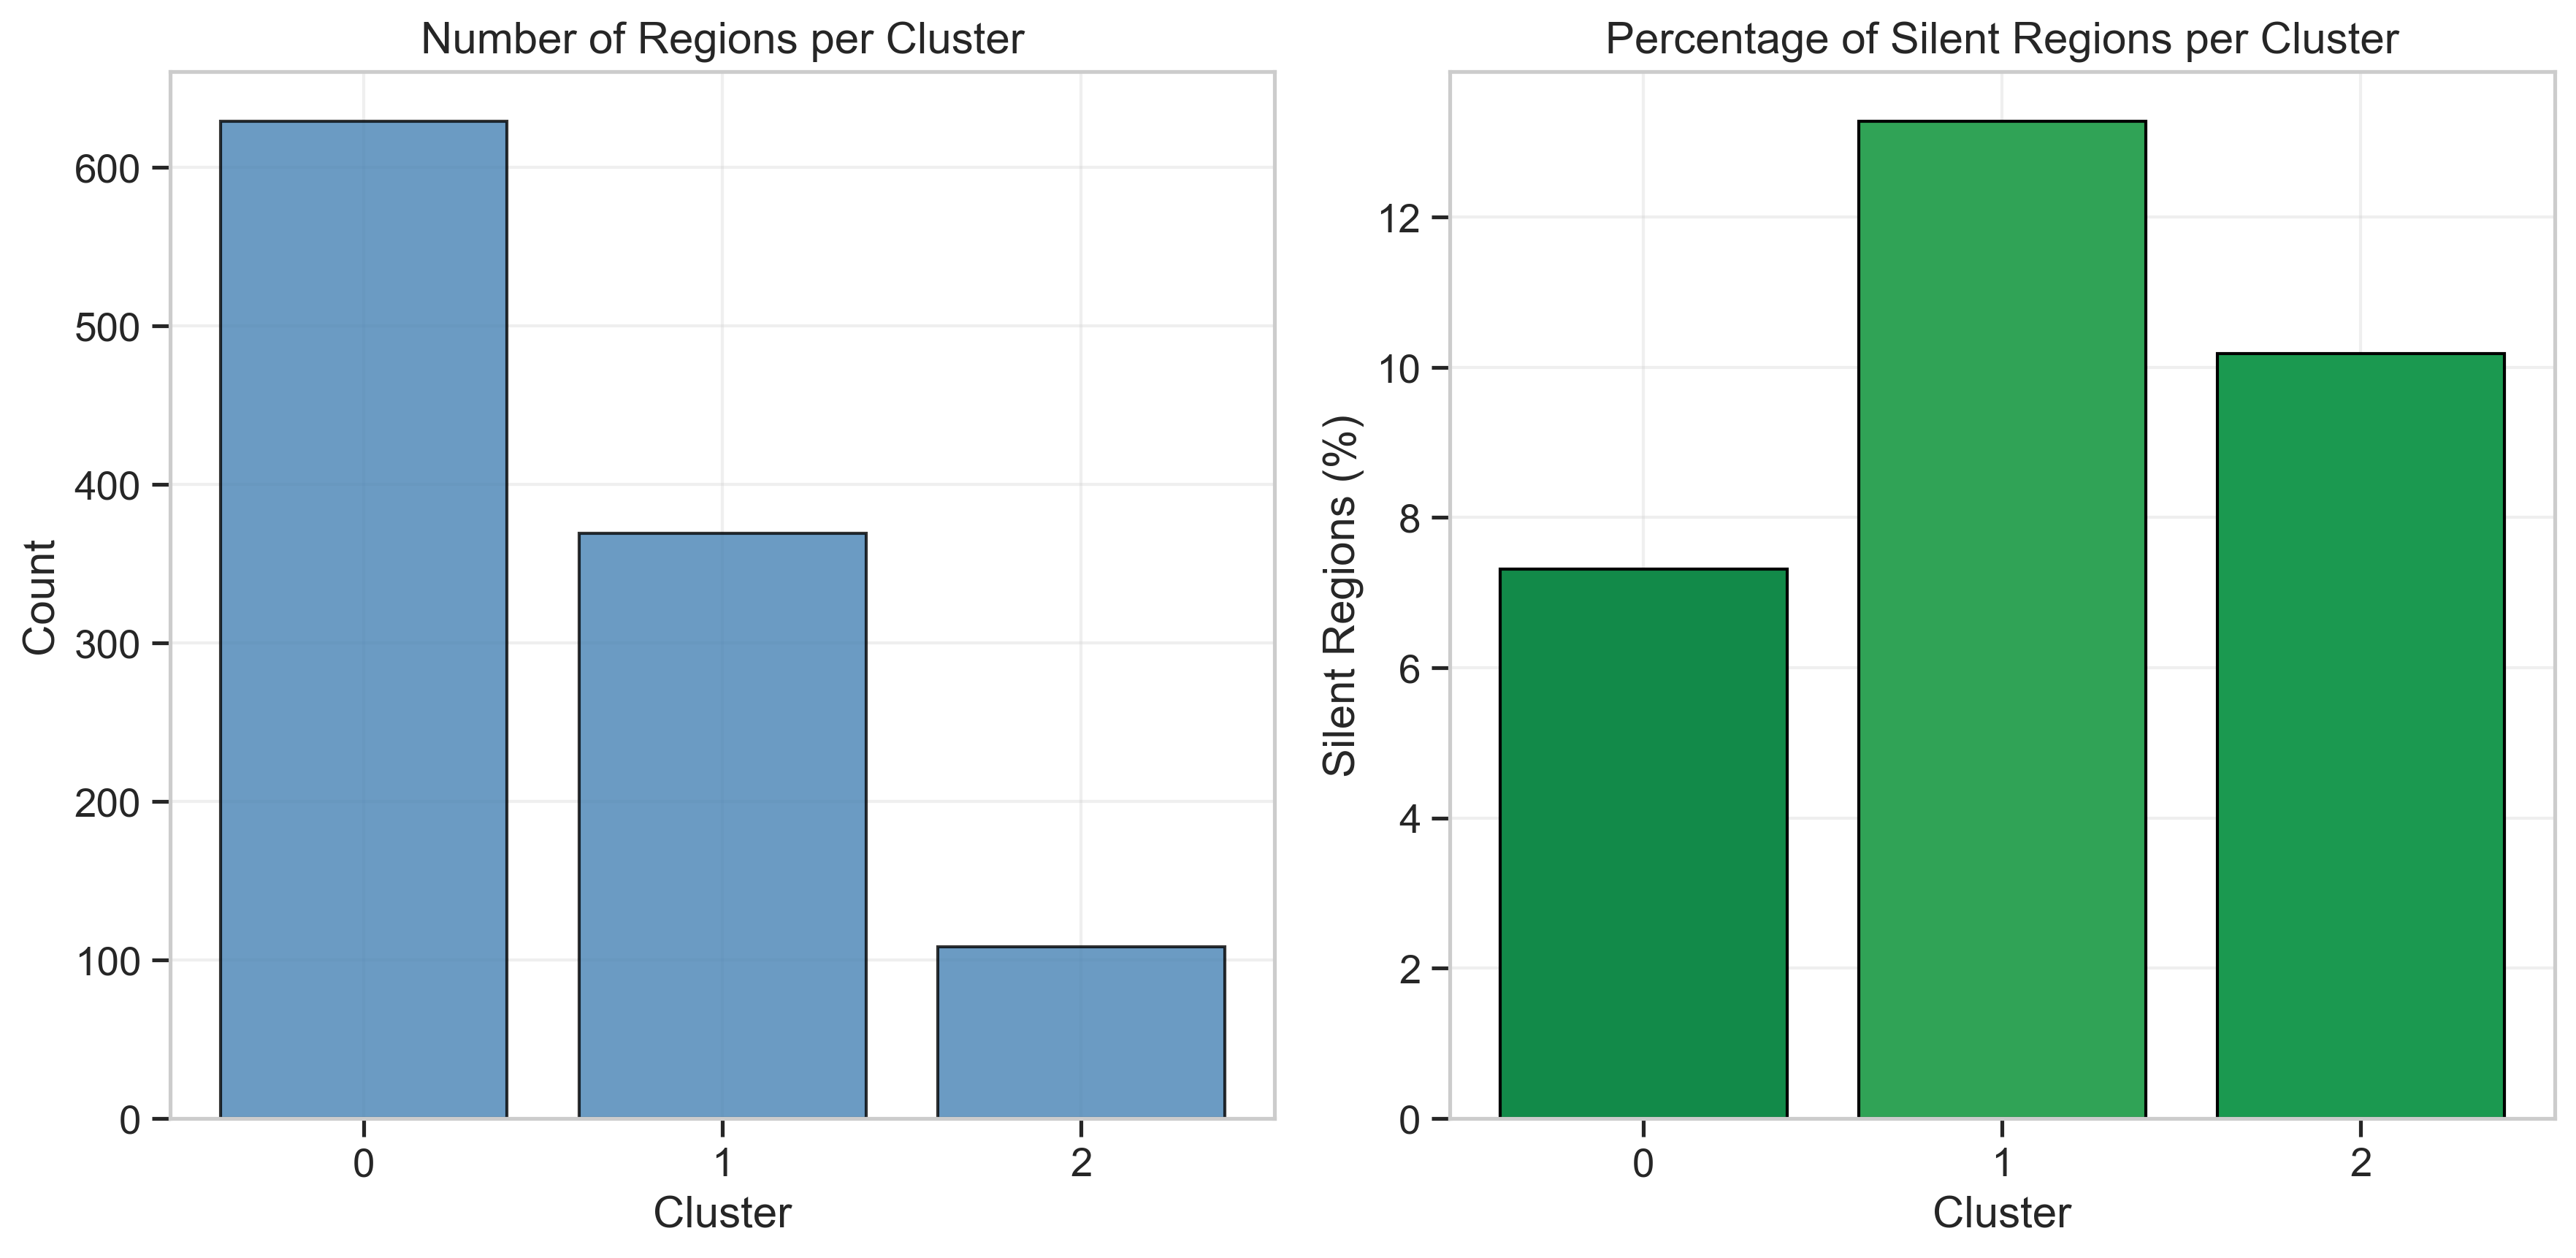
\includegraphics[width=0.95\textwidth]{cluster_composition.png}
    \caption{Left: Number of audio regions in each cluster. Right: Percentage of silent regions in each cluster.}
    \label{fig:cluster_comp}
\end{figure}

\subsection{Cluster Characteristics}

Analysis of the three clusters revealed distinct audio characteristics:

\begin{table}[H]
\centering
\begin{tabular}{>{\raggedright\arraybackslash}p{1.5cm} >{\raggedright\arraybackslash}p{4cm} >{\raggedright\arraybackslash}p{5.5cm} >{\raggedright\arraybackslash}p{3cm}}
\toprule
\textbf{Cluster} & \textbf{Size \& Silent \%} & \textbf{Common Annotations} & \textbf{Audio Characteristics} \\
\midrule
Cluster 0 & 629 regions (56.9\%) \newline 7.3\% silent regions & Beeps, cat meows, pedestrian crossing sounds, metallic impacts & High embedding values, predominantly sharp, distinct sounds \\
\midrule
Cluster 1 & 369 regions (33.4\%) \newline 13.3\% silent regions & Insect buzzing, dog barking, bass drums, human vocalizations & Low embedding values, more sustained sounds with less tonal clarity \\
\midrule
Cluster 2 & 108 regions (9.8\%) \newline 10.2\% silent regions & Hihat sounds, guitar playing, rhythmic claps, alarm-like sounds & High embedding values, musical and rhythmic sounds \\
\bottomrule
\end{tabular}
\caption{Characteristics of the three audio feature clusters}
\label{tab:cluster_chars}
\end{table}

Interestingly, silent regions were distributed across all three clusters rather than being concentrated in a single cluster. Cluster 1 had the highest percentage of silent regions (13.3\%), suggesting that this cluster might represent lower-energy or background sounds.

\subsection{Visualization with t-SNE}

To visualize the high-dimensional feature space, t-Distributed Stochastic Neighbor Embedding (t-SNE) was applied to project the data into two dimensions while preserving local relationships.

\begin{figure}[H]
    \centering
    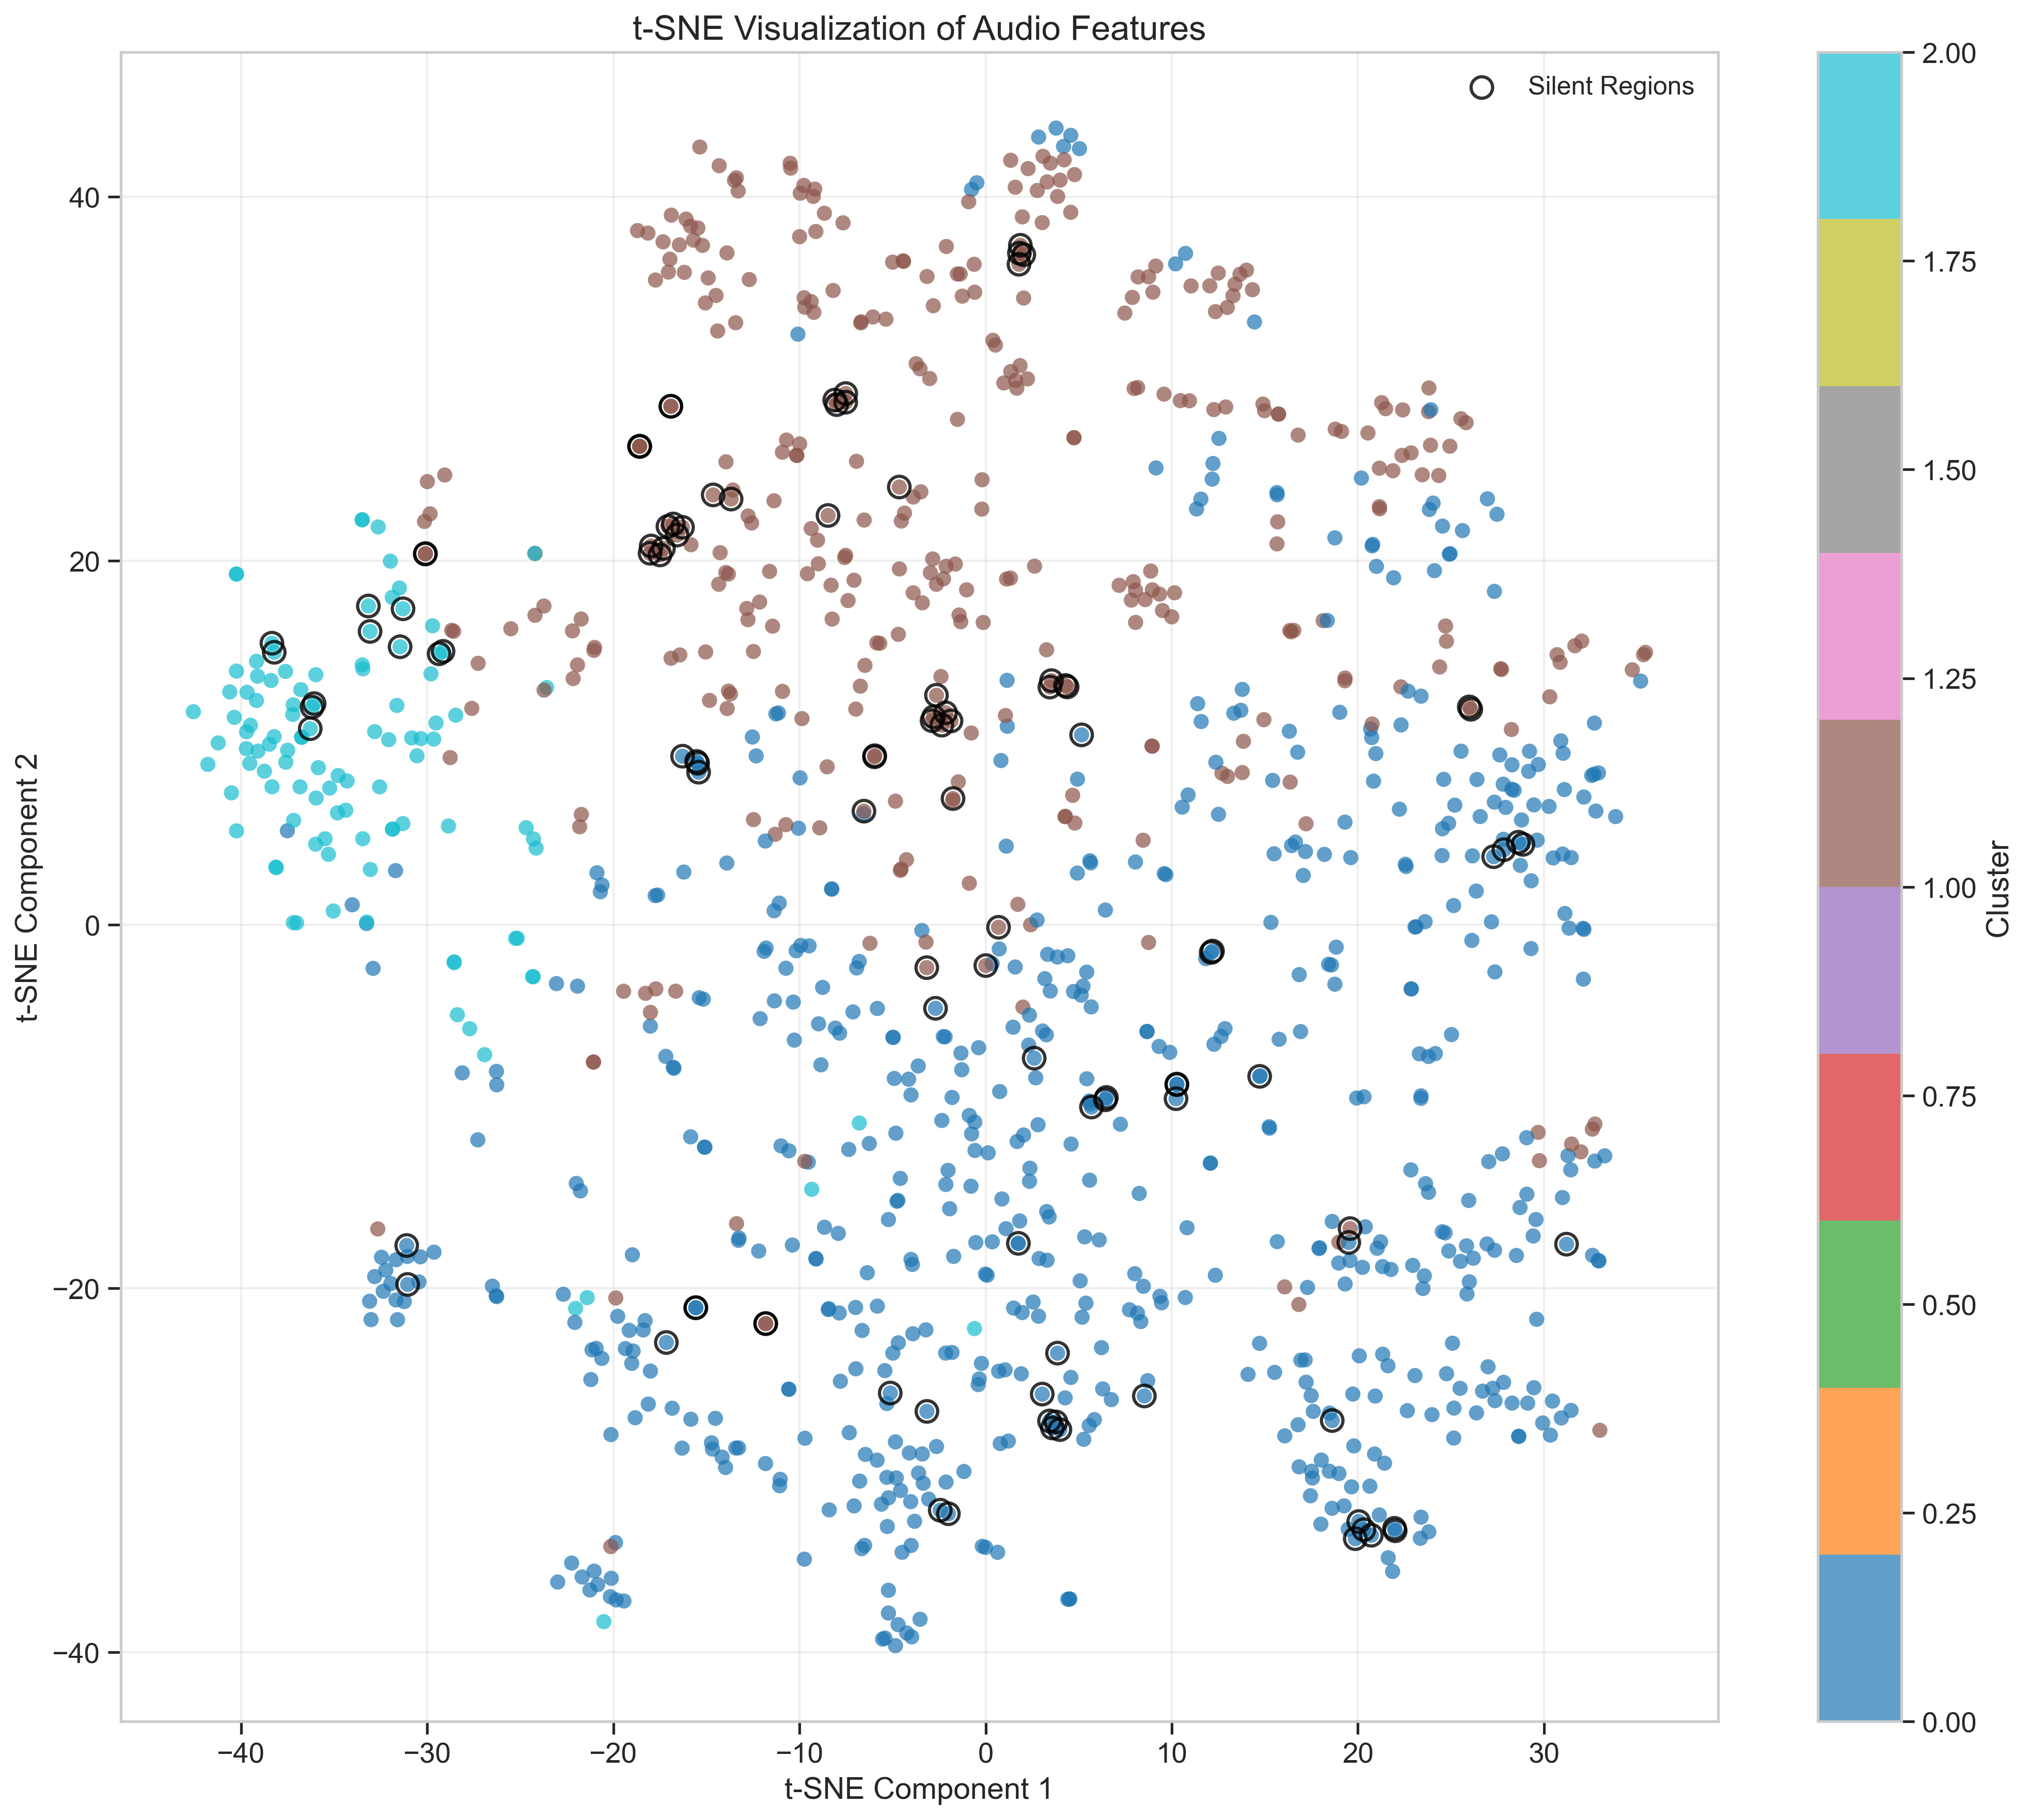
\includegraphics[width=0.8\textwidth]{tsne_visualization.png}
    \caption{t-SNE visualization of audio features colored by cluster assignment. Silent regions are highlighted with black circles.}
    \label{fig:tsne}
\end{figure}

The t-SNE visualization confirms the existence of distinct clusters in the audio feature space. However, it also shows that the boundaries between clusters are not always clear-cut, with some overlap between different sound types. Silent regions (marked with black circles) appear scattered throughout the feature space rather than forming their own distinct cluster, suggesting that the absence of sound is characterized differently depending on the context.

\section{Key Findings and Discussion}

\subsection{Dimensionality Reduction}
The dimensionality of the audio feature space can be significantly reduced (by 91.3\%) while preserving 80\% of the information.

\subsection{Important Features}

The most significant features for distinguishing different audio events are:
\begin{itemize}
    \item \textbf{Embeddings}: These learned representations capture good semantic content of the audio and account for the majority of the top features in principal components.
    \item \textbf{Mel spectrogram features}: Particularly in the lower frequency bands, these features provide important information about the energy distribution across frequencies.
    \item \textbf{MFCCs}: While fewer in number among the top features, the first MFCC (MFCC\_0) is particularly important as it relates to the overall energy of the signal.
\end{itemize}

\subsection{Audio Clusters}

Three distinct clusters of audio features were identified:
\begin{itemize}
    \item Cluster 0 (56.9\% of regions): Characterized by short, distinct sounds like beeps, meows, and impacts
    \item Cluster 1 (33.4\% of regions): Contains more continuous sounds like buzzing, barking, and sustained notes
    \item Cluster 2 (9.8\% of regions): Consists primarily of musical and rhythmic sounds
\end{itemize}

\subsection{Silent Regions}

Silent regions did not form a distinct cluster but were distributed across all three clusters, with the highest concentration in Cluster 1 (13.3\%). This suggests that silence is not uniform and may retain some characteristics of the surrounding audio context.

\section{Conclusion}

The audio feature analysis presented in this report provides valuable insights for developing sound event detection systems:

\begin{itemize}
    \item The original high-dimensional feature space (942 dimensions) can be effectively reduced to 82 dimensions while preserving 80\% of the variance.
    \item Mel spectrogram features, particularly in lower frequency bands, provide important information about energy distribution.
    \item Natural clustering of audio features reveals three primary groups of sounds with distinct characteristics.
    \item Silent regions show context-dependent properties rather than forming a single homogeneous group.
\end{itemize}

\end{document}